%%This is a very basic article template.
%%There is just one section and two subsections.

%%\RequirePackage[latin1]{inputenc}
\documentclass{article}
\usepackage{mathrsfs}
\usepackage[brazil]{babel}
\usepackage[utf8]{inputenc}
\usepackage{graphicx}
\usepackage{wrapfig}
\usepackage{boxedminipage}
\usepackage{amsmath}
\usepackage{yhmath}
\begin{document}

\newcommand{\observednet}{rede social observada} 

\title{NAIF: Network Analysis of Influence Framework}
\maketitle
\section{Introdução}

A análise de redes sociais tem sido utilizada para a investigação
de temas tão diversos quanto a difusão de inovações \cite{Coleman1966},
oportunidades de emprego \cite{Granovetter1995}, prevenção contra fraude
\cite{Neville2005} e marketing \cite{Domingos2001}. Muito dessa pesquisa inicial
se baseia em redes pequenas em torno de indivíduos escolhidos por amostragem
\cite{Wasserman}\cite{Newman2006}, porém a recente disponibilidade de informações
relacionais na internet através de sites de relacionamentos permitiu o
desenvolvimento da análise de redes em larga escala \cite{Boyd2007}. Não
obstante, o meio ainda carece de modelos dinâmicos de representação para redes
sociais observadas a partir do fenômeno digital \cite{Xiang2010} e é justamente
nesse ponto que o trabalho atual se concentra. Nosso objetivo é avaliar as
dificuldades, parâmetros e modelos existentes para a representação e modelagem
não-supervisionada de redes sociais digitais em larga escala e tempo real,
especificamente para aplicações que façam uso da rede para identificar atores
chaves em processos de difusão de conhecimento, inovações e recursos.

\section{Sobre Redes Sociais}

O estudo de rede sociais inicia nas décadas de 40 e 50, inicialmente voltado para
o estudo de pequenos grupos de individuos e suas interações, a rede era mensurada
através de observações, questionários e entrevistas \cite{Wasserman}.
Diferentemente de outras ciências sociais que consideravam apenas os indivíduo e
seus atributos, o estudo das redes sociais considera suas relações e os atributos
dessas relações. A rede social é um fenômeno complexo envolvendo os
relacionamentos de diversos atores em suas particularidades e que, através de um
processo que chamamos de mensuração, pode ser traduzido em uma representação.
Toda representação da rede social, por ser um modelo, é naturalmente parcial e
enviesado. Comumente, as pesquisas de redes sociais trabalham com grafos onde os
vértices são os atores e os arcos entre os vértices são as relações mensuradas; e
matrizes, onde as linhas e colunas são conjuntos de atores e que a posição
$(i,j)$ da matriz representa o arco \textbf{do} ator $i$ \textbf{para} o ator
$j$. Para economizar repetições, no decorrer deste trabalho quando estivermos nos
referindo ao fenômeno observado, utilizaremos o termo \textbf{\observednet},
enquanto que os termos \textbf{representação} e \textbf{rede social} serão
intercambiáveis.

Devido à disponibilidade de ferramentas matemáticas para o tratamento de grafos,
a análise de redes sociais desenvolveu-se rapidamente construindo métodos e
modelos estatísticos apropriados \cite{Butts2009}. A partir desse ferramental, o
ramo das ciências sociais passou a quantificar diversos fenômenos antes
considerados apenas do ponto de vista subjetivo, como a proeminência dos atores,
que estaria relacionada com a sua centralidade no grafo.

\subsection{$\bigotimes$ Alguma Formalização}

Representamos a rede como um grafo $G(V,E)$ onde $V$ é um conjunto de $n$
vértices (também chamados de atores) e $E$ o conjunto de arestas que os conectam.
Quando a representação é não-direcionada o par $(i,j)$ é chamado de aresta e
temos que $(i,j) \in E$ implica $(j,i) \in E$. No caso em que há direcionamento,
essa afirmação não se sustenta e por isso $(i,j) \in E$ não implica em $(j,i) \in
E$ necessariamente, além do que chamamos o par de arco de $i$ para $j$. De
maneira geral, sempre trataremos a representação como sendo direcionada.

Definimos a matriz de adjacência da rede $X$ com $n$ linhas e colunas, onde
$x_{ij} = 1$, se $(i,j) \in V$ ou 0 de outra forma. Essa matriz de $X$ é uma
representação binária da rede. Podemos generalizar essa notação para incluir
redes com valores discretos onde $0 \leq x_{ij} \leq m$ ou contínuos dispostos em
um intervalo. Ambas as notações, de grafo e de matriz, serão usadas de forma
intercalada neste trabalho.

\section{Redes sociais digitais}

Com a popularização da Internet é fato que pessoas se conectam umas às outras
virtualmente por seu intermédio. Os mecanismos de interação à disposição vão da
simples troca de mensagens, à venda e troca de produtos, à participação conjunta
em jogos \textit{multiplayer} massivos. Indo além do que sociólogo algum sonhou
realizar no início dos estudos de redes sociais, grande parte dessas interações
estão registradas, ou podem ser registradas eletronicamente a baixo custo,
fornecendo uma quantidade nunca antes disponível de informações para
estudos antropológicos e sociais da rede.

E assim tem sido, desde o nível micro com a análise dos conteúdos trocados
entre as interações pontuais de alguns indivíduos \cite{Recuero2008}, passando
por análise de potencial de marketing
\cite{Clemons2007}\cite{Domingos2001}\cite{Richardson2002}\cite{Ma2008}, busca
de pessoas \cite{ADAMIC2005}, de especialistas \cite{Ehrlich2007}, formação de
grupos \cite{Adamic2003}\cite{Backstrom2006}\cite{Kumar2006}, divulgação de
notícias \cite{Gruhl2004}, dinâmicas de prestígio
\cite{Salganik2006}\cite{Song2007}.

Enquanto nosso objetivo é alcançar resultados similares as pesquisas anteriores
de influência em redes sociais digitais, decidimos antes colocar a questão: como
mensurar a rede social digital? Cada pesquisa teve seu critério: quantidade de
e-mails trocados, recomendações, similaridades de perfil, participação nas mesmas
comunidades. Dissemos no começo que a \observednet é um fenômeno que pode ser
representado, mas que não é a representação em si, por esta razão, toda
representação carrega um \textit{bias}. Ora, ao acrescentarmos digital ao termo,
queremos dizer que estamos tratando da observação do fenômeno através de mídias
digitais; não mais das interações ao vivo e analógicas, mas através de
ferramentas eletrônicas que permitem a fácil armazenação, indexação e recuperação
dessa informação.

Para responder essa questão precisamos definir quais ferramentas são essas. Uma
resposta óbvia seria sites de relacionamento (ou sites de redes sociais),definido
como sendo um espaço (virtual) em que seja possível 1) criar um perfil, 2)
relacionar uma lista públicade amigos, 3) navegar por essa rede de perfis
interligados \cite{Boyd2007}. Porém tais sites são apenas um dentre muitos tipos
de ferramentas que podem ser analisados, como por exemplo: fóruns, listas de
discussão, sites de compartilhamento de conteúdo, comércio eletrônico,
\textit{blogs}, \textit{microblogs} (e.g., Twitter), salas de bate-papo. Por
questões de privacidade deixaremos de lado as formas pessoais de interação, como
\textit{instant messengers} e e-mails.

Ou seja, qualquer espaço (virtual) em que se é possível 1) identificar
unicamente um ator, 2) mapear atores agentes e receptores a uma determinada
interação com suas propriedades, pode ser insumo para a mensuração da rede. Mais
adiante veremos que idealmente também será necessário demarcar a posição dessa
interação no tempo, para possibilitar uma análise longitudinal da evolução da
rede. Chamamos de \textbf{medianeiro} qualquer espaço (virtual) que satisfaça a
condição acima.

Porque nos parece evidente a impossibilidade aplicar questionários ou entrevistas
com centenas de milhares de atores, respondemos a questão de como mensurar a rede
assim: através das interações encontradas nos medianeiros. A mensuração é um
processo de mineração de dados e, portanto, sujeita a todos os empecilhos típicos
do campo como informações incompletas, ruidosas, esparsas, redundantes. A questão
que nos aparece agora é como as interações observadas combinam-se para formar tal
rede e se ela é significativa para a análise de proeminência.

\section{Mensuração da rede}

\textit{Knowledge discovery} é o processo maior ``... não-trivial de identificar,
em dados, padrões válidos, novos, potencialmente úteis e ultimamente
compreensíveis'' \cite{Fayyad1996} e mineração de dados é uma de suas etapas.
Chamamos de mensuração da rede social digital o processo de minerar dados
proveninentes de meios digitais de interação social para formar uma
representação. Na última década alguns métodos norteadores para os projetos de
mineração de dados foram propostos, dentre os quais escolhemos o método de 6
passos descritos em \cite{Cios2005} e que consiste em sua forma geral:

\begin{description}
\item[1. Entendendo o domínio do problema]Neste passo devemos determinar os
objetivos do projeto e aprender sobre as possíveis técnicas conhecidas
para alcançá-los.
\item[2. Entendendo os dados]Este passo inclue coletar os dados, decidir quais
serão utilizados, priorizar atributos, verificar sua utilidade em relação aos
objetivos. Os dados precisam ser verificados em termos de completude,
plausabilidade, etc.
\item[3. Preparação dos dados]Este é o passo chave do qual o sucesso de todo o
processo depende; Ele geralmente consome metade de todo os esforço da mineração.
Aqui, decidimos quais dados serão usados como entradas para quais técnicas de
mineração do passo 4. O que pode envolver levantar amostragem de dados, executar
testes de correlação e significância, remoção e correção de ruído, etc. Os dados
tratados depois poderão serem processados para a seleção de características,
algoritmos de extração para redução da dimensionalidade dos dados, derivação de
novos atributos (discretização) e agregação dos dados (granularização). O
resultado é um novo conjunto de dados que atendem aos requesitos específicos
para servir de entrada às ferramentas de mineração selecionadas.
\item[4. Mineração dos dados]Aplicação dos métodos de mineração selecionados.
Apesar de ser através das ferramentas de mineração que as novas informações
são descobertas, sua utilização normalmente envolve menos esforço do que
preparar os dados. Ferramentas de mineração reunem diversos tipos de algoritmos
como conjuntos \textit{fuzzy}, métodos Bayesianos, computação genética,
aprendizado de máquina, redes neurais, etc. Para uma visão mais detalhada desses
algoritmos, nos referimos a \cite{JiaweiHan2006}.
\item[5. Avaliação do conhecimento descoberto]Interpretação dos
resultados, verificando a relevância da informação encontrada. Somente os
modelos aprovados são mantidos, todo o processo pode ser revisitado e ações
alternativas que levem à melhoria dos resultados podem ser identificadas.
\item[6. Usando o conhecimento descoberto]Entrega do conhecimento produzido.
Criação de um plano para monitorar sua utilização, documentação do projeto,
extender sua aplicação para outros domínios.
\end{description}

O método de 6 passos para mineração de dados foi escolhido dentre outros
possíveis devido ao seu viés acadêmico e modelo iterativo com ciclos de
\textit{feedback} explícitos que orientam o retorno a passos anteriores para a
melhoria do processo \cite{KURGAN2006}. Mostraremos agora, para cada passo do
método quais as considerações necessárias, dificuldades e possíveis soluções no
contexto da mensuração de redes sociais digitais para a análise da influência.

\section{Entendendo o domínio do problema}
\label{sec:ent_dom_pro}
No caso da análise da influência a mineração se divide em duas etapas a saber: a
mensuração da rede propriamente dita e o reconhecimento de atores chave. Da
segunda, depende a primeira. Caso a abordagem seja encontrar esses atores por
simulação ou por algoritmos de otimização, então a representação deve ter um
caráter probabilístico. Essa probabildiade pode ser inferida por um modelo a
partir de uma primeira representação bruta das interações ou gerado através de
propriedades comuns entre os atores. Por outro lado, existe a possibilidade de
utilizar técnicas da análise de redes sociais tradicional como métricas de
centralidade e prestígio para aproximar a influência do ator na rede. Nesse caso, a
representação utilizada para o cálculo dessas métricas não precisa ser
probabilística, mas também deve satisfazer alguns critérios que serão vistos
mais adiante.

Em \cite{Domingos2001}, os autores levantaram a questão: como selecionar o
conjunto ótimo de atores para a influência na rede? Demontraram que a solução
dessa questão é \textit{NP} e apresentaram três algoritmos de aproximação
considerando uma representação probabilística da rede. Depois deles, outros
vieram, mas todos voltados para modelos probabilísticos da rede. Devido a essa
dependência, achamos que é necessário uma atenção maior sobre a mensuração da
rede através de modelos probabilísticos devido a dificuldades que se
aprensentam, mas as considerações gerais que serão feitas não deixam de
se aplicar também para representações não probabilísticas.

\subsection{Dificuldades e critérios na mensuração}

Apesar dos algoritmos para aprendizagem de máquina e mineração de
dados estarem bem consolidados \cite{Cios2005}, a maioria deles não foram feitos
para dados relacionais. Algoritmos tradicionais de mineração de dados buscam
padrões considerando cada entrada de dados como independetes, mas dados
relacionais possuem o que chamamos de autocorrelação relacional.

Dados com autocorrelaçao relacional são aqueles em que as entradas possuem
correlação entre si a depender de uma relação comum. Em ciências sociais, essa
autocorrelação pode ser fruto de uma propriedade chamada de homofilia e que
pode ser vista de maneira simples como pessoas parecidas tendem a formar laços
e vice versa. Recentemente, algumas técnicas de mineração de dados tem sido
desenvolvidas para tratar dados relacionais como os modelos relacionais
probabilísticos, classificadores Bayesianos de primeira ordem e árvores de
probabilidades relacionais \cite{Jensen2002}. Técnicas mais antigas incluem
programação de lógica indutiva e a análise de redes sociais tradicional.

Recentes trabalhos na área utilizam de diversos tipos de interação para a
mensuração da rede como por exemplo a similaridade entre classificação de
produtos \cite{Richardson2002}, similaridade em termos extraídos de mecanismos de
busca na internet \cite{MATSUO2007} e co-autoria em artigos científicos
\cite{Kempe2003}. Em \cite{Xiang2010} temos uma mensuração combinando diversas
interações observadas nos sites de relacionamento Facebook e LikedIn, que
possuem propostas diferentes de utilização. A existência ou ausência de cada
interação, como a recomendação, troca de mensagens, marcação em fotos, é reunida
em um vetor binário. Da mesma forma, a similaridade entre os atores é reunido em
outro vetor binário, onde cada dimensão representa uma propriedade comparada e
recebe 0 caso seja diferente, 1 se igual. A partir de então, os autores propõem
um modelo de força da relação como variável escondida com causa na similaridade
e com consequência na interação. 

Para a relação força e interação os autores propõe um modelo discriminativo que
possibilita o calculo da probabilidade condicional da interação a partir da
força da relação, isso é feito por amostragem da população. Essa estimativa é
usada para calibrar um modelo generativo que relaciona a similaridade à força da
conexão, que é utilizado por sua vez para calcular a força entre dois atores
quaisqueres. Essa combinação de modelo discriminativo e generativo possibilita a
inferência não supervisionada da força do laço, o que é um ponto positivo para
esta abordagem, porém ela subestima outros fatores igualmente importantes.

A similaridade é apenas uma das possíveis componentes da força da conexão,
propriedade conhecida como homofilia. Para um entendimento de um processo geral
de mensuração da rede digital, precisamos remontar a um dos trabalhos fundantes
da análise de redes sociais onde Granovetter lança, pela primeira vez, a
hipótese:

\begin{quotation}\textit{
A força da conexão [entre dois atores] é uma combinação
(provavelmente linear) da quantidade de tempo, intensidade emocional,
intimidade (confidência mútua) e serviços recíprocos que a
caracterizam.} \cite{Granovetter1973}
\end{quotation}

Granovetter também separa indicadores de pescritores, indicadores são
componentes de fato da força da conexão, enquanto que prescritores são
contigências contextuais que influenciam, mas não são componentes. Dentre os
prescritores está a homofilia, o que quer dizer que a similaridade entre os
atores influencia a conexão, mas é a intensidade, duração, intimidade e
reciprocidade que indicam a sua força. Dessas quatro dimensões iniciais
(tempo, intensidade, intimidade, reciprocidade), acrescentaram-se nove outras no
decorrer de três décadas de pesquisa. Na Tabela \ref{tab:resumao} temos um
apanhado dos indicadores propostos na literatura. 

Em \cite{Gilbert2009} encontramos uma análise da composição desses indicadores na
força da conexão. Através de um modelo discriminativo os autores encontram a
correlação linear entre 74 variáveis em cima das interações coletadas no site de
relacionamento Facebook e a força da relação coletada através de questionário com
uma amostra de 32 indivíduos. Sua análise leva em consideração sete indicadores
de força, separando as variáveis em dimensões do tipo intensidade, intimidade,
duração, reciprocidade, estrutural, emocional, similaridade. É interessante
notar que duas dimensões escolhidas são consideradas como prescitoras da força e
não indicadoras, que são a estrutura e a similaridade. Sobre similaridade já
falamos, já as variáveis estruturais referem-se a padrões da rede como a
transitividade, i.e., amigo de amigo seu tem maior chance de ser seu amigo
também.

Os resultados mostram uma partição da força por dimensão que pode ser vista na
Figura \ref{fig:forca}. As dimensões de intimidade, intensidade e duração são as
três maiores componentes da força. As variáveis de estrutura, sozinhas, são as
que menos utilidade tem para a previsão da força, porém quando analisada em par
com outras dimensões demonstram alto de grau de interação. Nas palavras dos
autores:

\begin{quotation}
\textit{A dimensão estrutural possui um papel menor como fator linear.
Entretanto, ela possui um papel regulador importante através dessas interações
[com as outras dimensões]. Uma forma de interpretar este resultado é que
interações individuais importam, porém elas são filtradas através do
clique\footnotemark de amigos antes de impactar a força da
relação.}\cite{Gilbert2009}
\end{quotation}

\footnotetext{clique pode ser traduzido como grupo de amigos com interesses
similares e que são vistos por outros como exclusivistas; panelinha.}

\begin{figure}[h!]
  \caption{Poder preditivo das sete dimensões da força da conexão}
  \centering
    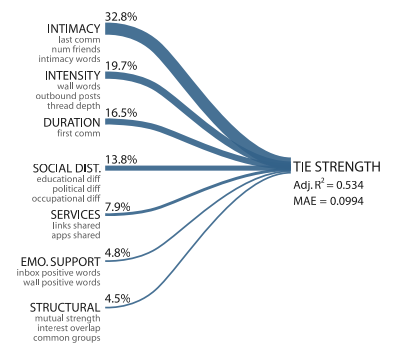
\includegraphics[width=0.7\textwidth]{imgs/composicao-forca.png}
    \label{fig:forca}
\end{figure}

Esse resultado confirma o papel prescritivo das variáveis estruturais. Não
obstante os resultados, o método de \cite{Gilbert2009} possui restrições quanto a
utilidade em nosso cenário digital. Em primeiro lugar, sua abordagem
supervisionada não escala com a rede e não há estudo sobre o erro induzido pela
amostragem. Em segundo lugar, o tipo de conexão não é direcionado, isto é, ambos
atores conferem o mesmo valor para a relação. Essa simplificação é nociva para o
nosso objetivo de análise de influência, já que a assimetria de influência é
bastante comum, por exemplo, um aluno pode ter grande consideração por um
professor, mas o inverso em pé de igualdade raramente é verdade.

\begin{table} [htbp]
	\large       % tamanho da fonte 
	\setlength{\arrayrulewidth}{2\arrayrulewidth}  % espessura da  linha
	\setlength{\belowcaptionskip}{10pt}  % espaço entre caption e tabela
	\caption{\textit{Sumário dos componentes da força da conexão}
	\cite{Petroczi2006}} \centering   % tabela centralizada
	\begin{tabular}{| p{5cm} | p{4cm} |}
	\hline
	\textbf{Dimensão} & \textbf{Referências} \\ \hline\hline
	Frequência & \cite{Benassi1999}, \cite{Blumstein1988}, 
	\cite{Granovetter1995}, \cite{Marsden1984}, \cite{MATHEWS1998},
	\cite{Mitchell1987}, \cite{Perlman1987} \\\hline
	Intimidade & \cite{Blumstein1988}, \cite{Marsden1984}, \cite{MATHEWS1998},
	\cite{Mitchell1987}, \cite{Perlman1987}\\\hline
	Investimento voluntário na relação & \cite{Blumstein1988},
	\cite{Perlman1987}\\\hline
	Aconselhamento dado e recebido & \cite{MATHEWS1998}\\\hline
	Desejo de companhia & \cite{Blumstein1988}, \cite{Perlman1987}\\\hline
	Multiplicade dos contextos em que há interação & \cite{Blumstein1988},
	\cite{Granovetter1973}, \cite{Marsden1984}, \cite{Perlman1987}\\\hline
	Duração & \cite{Blumstein1988}, \cite{Granovetter1973}, \cite{Marsden1984},
	\cite{Perlman1987}\\\hline
	Reciprocidade & \cite{Blumstein1988}, \cite{Friedkin1980},
	\cite{Granovetter1973}, \cite{MATHEWS1998}, \cite{Perlman1987}\\\hline
	Suporte	emocional (intensidade) & \cite{Blumstein1988},
	\cite{Granovetter1973}, \cite{Mitchell1987}, \cite{Perlman1987},
	\cite{Wellman1982}, \cite{Wellman1990}\\\hline
	Confiança & \cite{Granovetter1973}, \cite{Marsden1984},
	\cite{MATHEWS1998}\\\hline
	Sociabilidade & \cite{Mitchell1987}\\
	\hline
	\end{tabular}
	\label{tab:resumao}
\end{table}

Isso nos leva a reflexão de que, para análise de influência, a utilização de
todas as dimensões da força da conexão pode ser muito restritiva. Uma delas, como
no exemplo já citado, é a dimensão de reciprocidade: um ator com prestígio exerce
grande influência sobre seus admiradores, mas cada admirador individualmente não
consegue exercer influência de igual intensidade sobre ele. Outro exemplo são os
indíviduos de fronteira, que se conectam à periferia de dois grupos; as suas
conexões são fracas, mas exerce grande influência na transferência de
conhecimento entre os grupos. Daí temos que apesar da noção de força de
Granovetter está relacionada com a influência, ela não é condição necessária
\cite{Brown2007}.

Finalmente, nenhuma das soluções estudadas considera a evolução da rede no
tempo. Nesse aspecto algumas pesquisas utilizam fotografias na rede em
momentos diferentes ou agregações das interações por período. A partir daí
utiliza-se modelos probabilísticos \cite{Sarkar2005}, meta-grupos
\cite{Berger-Wolf2006} ou modelos provenientes da psicologia comportamental e da
administração \cite{Brelger2004}. Nenhum deles, entretanto, é combinado com
a teoria da força das relações para permitir sua aplicação em processos de
mensuração de redes sociais digitais.

A partir de então sugerimos alguns critérios para as ferramentas de mineração
que serão usadas no processo de análise de influência:

\begin{enumerate}
  \item Deve ser não supervisionada para aumentar a chance de escalar com o
  tamanho da rede;
  \item Deve considerar a força das relações na maior quantidade possível de seu
  espectro de componentes. Por tanto, a representação resultante não deve ser
  binária;
  \item Deve também levar em consideração aspectos estruturais da rede como
  transitividade e \textit{brokerage};
  \item Deve ser longitudinal, isto é, incorporar o elemento tempo na análise,
 levando em conta a formação e dissolução de relações, entrada e saída de
 atores;
\end{enumerate}

Uma vez escolhida as ferramentas de mensuração e análise, devemos agora passar
para o passo seguinte e selecionar quais dados serão usados e se são válidos.

\section{Entendendo os dados}

A primeira crítica que deve ser avaliada é a de que interações digitais não são
um indicador confiável da relação entre dois indivíduos \cite{Clemons2007}. Que
se um amigo virtual não é mais do que um conhecido, não há relação de influência
significativa entre eles. Porém, as pesquisas em redes sociais digitais tem
demonstrado que em sua maior parte, os indivíduos utilizam os meios digitais para
continuar uma relação já existente no mundo \textit{off-line}
\cite{Haythornthwaite2005} \cite{Recuero2008} \cite{Sassen2002}. Outra vantagem
de ater-se a interação observada é que ela não carrega alguns pontos fracos da
abordagem direta (questionário, entrevista) que é o esquecimento e a omissão das
relações nas respostas (a taxa de erro quando interrogados sobre as interações
que mantiveram chega a 50\% em comparação com a observação) \cite{Mislove2007}.
Mas a vantagem mais óbvia e determinante é o custo, coletar e processar os dados
advindo das interações dos atores no meio digital é muito mais barato que fazer o
mesmo para interações não digitais, na medida em que o tamanho da rede aumenta,
ou mesmo em comparação com entrevistas e questionários. Na casa dos milhões de
membros na rede, qualquer coisa que não seja a primeira opção é atualmente
inviável.

Nessa etapa da mineração, uma vez delineada as técnicas de mensuração, é
necessário escolher quais medianeiros serão utilizados. Recapitulando a definição
de medianeiro: é todo espaço (virtual) em que seja possível 1) definir unicamente
um ator, 2) mapear atores agentes e recepetores a uma interação e suas
propriedades. Alguns exemplos são: salas de batepapo, fórums, lista de discussão,
sites de relacionamentos, sites de compartilhamento de fotos e vídeos. Para cada
medianeiro, o pesquisador pode ter maior ou menor acesso à informação.

Quando a única informação disponível são as publicadas nas páginas da internet
ou outros meios de acesso ao medianeiro, dizemos que sua análise é
\textbf{extrínseca}. A grande maioria dos trabalhos em redes sociais digitais
hoje é feito dessa forma com a confecção de \textit{crawlers}, programas de
computador que percorrem conteúdos \textit{on-line} retirando informações
estruturadas de dados semi-estruturados próprios para o uso humano, como as
\textit{web pages}. Esse tipo de análise é limitada muitas vezes à interação
presumida, já que geralmente através dela é possível saber que um ator publicou
conteúdo na comunidade, mas não quem da comunidade parou para vê-lo.

Quando as informações são coletadas diretamente dos banco de dados do
medianeiro, chamamos essa análise de \textbf{intrínseca}. A análise intrínseca
encerra diversas vantagens, principalmente por ter acesso ao funcionamento da
rede, podendo coletar dados sobre seu uso. São informações como mensagem lidas e
não lidas, tempo usado em cada uma, e que formam um tipo de interação que
chamaremos de \textbf{passiva}.

Porém muitos são os tipos de interação digitais encontradas e enquanto não
tivermos um maior entendimento das suas semelhanças e diferenças, não nos será
possível construir uma abordagem integrada de mensuração. Por uma tipologia das
interações digitais é então que nossa atenção deve agora se voltar.

\subsection{Por uma tipologia das interações digitais}

O estudo das interações humanas é o objeto das ciências sociais, notadamente, no
contexto micro, da antropologia e etnografia. Somente com a popularização da
internet é que as interações digitais (mediadas por computador) ocuparam maior
destaque nesse meio \cite{Wellman1996}\cite{Herring2002}. Uma tipologia inicial
foi proposta em \cite{Burnett2000} e revisada em \cite{Burnett2004}, porém o
seu foco é na distinção entre interações direcionadas e as não-direcionadas para
a aquisição de informação. Nossa tipologia começa dela, mas expande incorporando
conceitos de capital social \cite{Recuero2008} e abrangência
\cite{MARTINEZ2000}.

Podemos as interações digitais dividir por tipo do \textbf{conteúdo},
\textbf{abrangência} e \textbf{intenção}. Os tipos de conteúdos podem ser
divididos em dois grandes grupos: textuais e não textuais. Abrangência consiste
se a interação é individual básica, individual desenvolvida, individual
generalizada ou comum. Finalmente, quanto a intenção podemos classificar a
interação em afirmativa, negativa, conversacional, informativa, conectiva. É
importante ter em mente que as categorias apresentadas não são, de forma alguma,
mutuamente exclusivas, podendo mesmo numa interação singular ser combinadas em
diferentes formas.

\subsubsection{Por conteúdo}

O tipo do conteúdo da comunicação diz muito sobre o capital social que carrega
\cite{Kim2007}, por exemplo, mensagens síncronas possuem vocabulário mais
limitado, são mais informais e possuem maior carga social fática
(\cite{Danet1998}, \cite{Ko1996}, \cite{WERRY1996}; \textit{Apud}
\cite{Herring2002}) enquanto que mensagens assíncronas tendem a ser maiores,
mais multifuncionais e linguisticamente complexas (\cite{Herring1999};
\textit{Apud} \cite{Herring2002}). De acordo com essas diferenças, mensagens
síncronas parecem ser mais apropriadas para a interação social enquanto que
mensagens assíncronas o são para discussões mais complexas e resolução de
problemas.

Também não é nosso objetivo ainda nos aprofundarmos numa análise do discurso
mediado por computador \cite{Herring2001}. A classificação que utilizaremos 
aqui usa o conceito de protótipo e por tanto tem expressividade reduzida diante
do surgimento de formas interação inovadoras \cite{Herring2007}. Porém ela será
suficiente nesse estudo inicial sobre mensuração de redes para a combinação de
diferentes interações. Dividimos inicialmente em duas grandes categorias:
textual e não textual; para cada uma então são listados seus principais
protótipos.

\begin{description}
\item[conteúdo textual] Já foi dito o quanto o texto é importante para a
comunicação mediada por computador, mesmo numa época em que o compartilhamento
de vídeos está na moda, o texto, na forma de comentários, continua sendo o
principal móvel das trocas sociais \cite{Herring2002}. São desse tipo:
\begin{itemize}
  \item comentários
  \item mensagens
  \item tópicos
  \item \textit{blogs} e similares
  \item \textit{microblogging} e similares
  \item descrições
\end{itemize}
\item[conteúdo não-textual] Nesse grupo estão relacionados não só as interações
áudiovisuais, mas também as interações ``mudas'' como a formação de laços
explícito entre os atores, a classificação mútua dicotômica ou graduada e a
recomendação de conteúdos de terceiros. Exemplos:
\begin{itemize}
  \item fotos
  \item vídeos
  \item \textit{links}
  \item laços explícitos entre os atores
  \item classificação (\textit{rating}, \textit{ranking}, favoritos)
  \item compartilhamento
\end{itemize}
\end{description}

\subsubsection{Por abrangência}

A abrangência define quais são os atores influenciados pela interação, em
outras palavras, os participantes do ``discurso" \cite{Dooley2001}. É através da
abrangência da interação que o processo de mensuração recupera os atores
participantes na conexão mensurada e por tanto representa a forma como os
agentes buscam se posicionar na rede como um todo. Essa classificação foi
apresentada uma primeira vez em \cite{MARTINEZ2000}.
\begin{description}
\item[individual básica] Classificam-se neste grupo as interações de caráter
privativo que partem de um ator específico para outro ator. As interações que
tipicamente pertencem a este grupo são as mensagens, os pedidos de conexão e o
compartilhamento de conteúdo do tipo ``\textit{forward}''.
\item[individual desenvolvida] Quando a interação se inicia em um ator e envolve
sua rede imediata de contatos sem estar publicamente disponível para qualquer
membro da rede. São desse grupo, em sua maioria: tópicos de fóruns, fotos,
vídeos, compartilhamentos, microblogging.
\item[individual generalizada] Quando a interação se inicia em um ator e
torna-se pública para todos os atores da rede. Todos os tipos de interação podem
se classificar nesse grupo, depende do grau de livre acesso que a rede
proporciona aos seus membros.
\item[comum] Quando a interação se dá num espaço de igualdade, quer dizer, que
todos podem interagir com todos no mesmo nível, chamamos de interação comum. Um
exemplo claro dessa categoria é as salas de batepapo onde todos podem publicar
mensagens para todos lerem. Listas de discussão também seguem esse modelo.
Um \textit{Blog} em particular não é uma interação comum, na maioria dos casos,
porque só o mantenedor do \textit{blog} pode publicar artigos nele, já o
espaço de comentários do artigo possa ser considerado um espaço comum.
\end{description}

\subsubsection{Por intenção}

Por último, mas não por menos, temos a intenção sobre a qual o ator reveste sua
interação. A diferença de intenção não só pode representar mudança significativa
na força da influência, como necessariamente define os possíveis resultados da
interação. Em \cite{Recuero2008} encontramos uma classificação da intenção
das interações, que para o escopo proposto por esse trabalho é suficiente e as
divide em cinco grandes grupos:
\begin{description}
\item[afirmativa] Trata da afirmação de suporte social entre um ator e outro.
Pode ser um comentário positivo relacionado a uma interação prévia do ator
elogiado, uma avaliação positiva, a recomendação do seu conteúdo para outros.
\item[negativa] Quando a interação se dá para depreciar o outro. Pode ser por
comentário, tópicos, mensagens, avaliação negativa.
\item[conversacional] Quando a interação tem caráter pessoal, relacionado a uma
conversação que se inicia ou que está em andamento.
\item[informativo] Quando a intenção é informar um grupo de atores sobre
determinado assunto. Avisos, artigos, propaganda, críticas.
\item[conectivos] Quando a intenção é formar laços explícitos através da rede.
Pedidos para conexão como adicionar à lista de contatos/amigos/etc.
\end{description}
Das três dimensões de classificação da interação, a intenção é certamente a mais
difícil de aferir computacionalmente. Isso porque sua característica subjetiva o
que a torna também objeto ideal para a pesquisa qualitativa. Porém recente
evolução da mineração de opinião e análise de sentimentos pode trazer opções
para a análise de intenção no contexto da mensuração das redes sociais digitais.
Para uma compilação dos principais avanços e desafios na área, nos referimos a
\cite{Wilson2005}, \cite{Ding2007} e \cite{Pang2008}. Por sua importância e
dificuldade, teremos o cuidado de anotar mensurações de redes sociais digitais
que não levem em consideração a intenção, como \textbf{análises ingênuas}.

\subsubsection{Interações passivas}

Para finalizar essa seção sobre interações, falaremos aqui de interações passivas
e comportamentais que podem levar a um maior entendimento de como o ator investe
sua atenção na rede e, por isso mesmo, como se posiciona na rede em relação a
outros atores. Podemos considerar como interação passiva como aquela que não é
necessariamente percebida pelos outros atores além do interagente, nesse tipo
encontram-se todas as interações do ator com o sistema como: mensagens lidas, não
lidas, tempo usado para cada mensagem, perfis visitados, tempo usado na leitura
de outros conteúdos. Essas informações poderiam ser utilizadas numa análise
intrínseca da rede para a concepção de um modelo mais real do interagente quanto
ao dispêndio da atenção.

\subsubsection{$\bigotimes$ Notação}

Seja $\mathscr{X}$ um medianeiro, existirá um conjunto $\mathscr{L}$ de
interações associado a $\mathscr{X}$. Considere o conjunto $\mathscr{N}$ de
atores envolvidos através do medianeiro $\mathscr{X}$. Temos que para cada
iteração $l_k \in \mathscr{L}$ existe pelo menos um ator $n_i \in \mathscr{N}$
que provocou a interação, chamamos esses atores de agentes ou autores. Também
existe pelos menos um ator $n_j \in \mathscr{N}$ que recebeu a interação,
chamamos esses atores de receptores, audiência ou abrangência. Assim para fins de
notação, sendo $\mathscr{P}(.)$ o conjunto das partes, considere
$A:\mathscr{L}\to\mathscr{P}(\mathscr{N})$ onde $A(l_k)$ é conjunto de autores de
$l_k$. Da mesma forma, faça $R:\mathscr{L}\to\mathscr{P}(\mathscr{N})$ onde
$R(l_k)$ é conjunto de receptores de $l_k$. Nenhuma das duas funções são
inversíveis, porém para economizar a notação definimos
$A^{-1}:\mathscr{N}\to\mathscr{P}(\mathscr{L})$ onde $A^{-1}(n_i)$ é o conjunto
de interações $l$ tal que $n_i \in A(l)$. O mesmo deve ser considerado para
$R^{-1}$.

\subsection{Uma teoria da atenção como capital social}

Antes de prosseguir para a etapa seguinte na mensuração da rede, gostaríamos de
discutir uma aproximação para a influência entre os atores: atenção como
capital social. Capital social é todo recurso que mantém a rede social
\cite{Coleman1988} e pode ser mobilizado através das conexões
\cite{Gyarmati2004}. Exemplos de capital social são a confiança e o suporte
emocional. Por esta razão uma outra forma de chamar as dimensões de força da
conexão de Granovetter é de capital social, i.e., quanto maior o fluxo de
capital social que a conexão suporte, maior é a sua força. Mostraremos que a
atenção não só atende a definição de capital social, como se aproxima mais do
conceito de influência e, certamente, é mais fácil de medir.

Foi o vencedor do prémio nobel, o economista Herbert Simon, que disse:

\begin{quotation}\textit{What information consumes is rather obvious: it consumes
the attention of its recipients. Hence a wealth of information creates a poverty
of attention }\cite{Simon1996}
\end{quotation}

Vivemos em uma era de riqueza de informação e por esta razão estamos em escassez
de atenção \cite{Goldhaber1997}. Atenção é vista atualmente como \textbf{o} mais
importante recursos para as organizações \cite{Davenport2001}. Ela também assume
papel crucial na formação e manutenção de relacionamentos e como é um recurso
limitado, o mais comum é que cada um invista nas relações que percebam ser mais
importantes \cite{Dindia1993}. Por esta razão a atenção satisfaz os critérios de
capital social, a saber 1) contribuir na manutenção da rede, 2) pode ser
mobilizada através das conexões. Vários estudos consideram a atenção como a nova
economia na internet, através de comentários, classificações positivas e
\textit{profiles} \cite{Humphreys2009} \cite{Wu2009} \cite{Skageby2009}. Nessa
economia nós temos ``celebridades'' e ``fãs'', muito similar ao que encontramos
no contexto da influência.

Na verdade somente o fato de prestar atenção em si já é uma influência per si,
independente das futuras escolhas do receptor. Em uma pesquisa em Parma, na
Itália, por volta de 1991, neurocientistas conectaram cabos ao cérebro de macacos
de forma que o computador reconhecia pelo padrão de ativação dos neurônios quando
ele levava um amendoin à boca. Não obstante a ativação fosse registrada
eletrônicamente, eles também ligaram o aparato a um auto-falante de forma que
mesmo estando distantes soubessem quando o evento acontecia. Quando um aluno
passou pelo laboratório e levou uma banana à boca, o alarme soou. Porém o macaco
não estava fazendo nada além de observar o estudante. Estava claro que a atenção
no gesto do estudante disparava o cérebro a reproduzir (em sua mente) o movimento
como se fosse seu (\cite{Rizzolatti1996};\textit{Apud} \cite{Goldhaber2006}).

Resta-nos saber como mediremos a atenção. Ora, em qualquer interação o que é
trocado em primeiro lugar entre o agente e os receptores é atenção. A atenção
flui não só do receptor para o agente ao receber a ``mensagem'', no que chamamos
de atenção \textbf{direta}, mas também do agente para os receptores, por a ter
preparado e comunicado, que chamamos de atenção \textbf{residual}
\cite{Goldhaber1997}. Apesar de que em quantias bem menores proporcionalmente,
por que o que cada receptor recebe é uma atenção ilusória, é uma fração da
atenção do agente e que o satisfaz de alguma forma na interação de modo que para
ele parece um bom negócio continuar retribuindo-a com a sua. Mas como essa
atenção se relaciona com as dimensões da força de Granovetter? Para responder
essa questão precisaremos usar nossa tipologia da interação.

Em primeiro lugar, frequência e duração são dimensões temporais que são
recuperadas a partir do tratamento longitudinal da rede. A frequencia das
interações e data do começo delas são métricas simples de colher e que contribuem
para força total. Quanto a intimidade, podemos verificar que a depender da
abrangência teremos espaço para maior ou menor intimidade, ou seja, quando mais
restrito a abrangência mais íntima a interação, sendo a mensagem de pessoa a
pessoa a forma mais íntima possível. Quanto a carga emocional, mesmo não tendo à
disposição meios de análise de sentimento, sabemos que as interações que mais nos
chamam atenção são as que possuem carga emocional \cite{Davenport2001}. Daí
podemos aproximar a dimensão de suporte emocional por uma combinação da de
duração, frequência e intensidade.

Para finalizar nossa consideração sobre a atenção como capital social, é
importante mencionar que a atenção não é direcionada apenas sobre um foco, mas
sobre o contexto. Isto quer dizer que alguns indivíduos podem receber atenção
indiretamente terem sido citados, por intermediarem a interação ou por
simplesmente fazer parte do contexto de alguma forma. Essa atenção chamamos de
\textbf{transitiva}.

\subsubsection{$\bigotimes$ Formalização}

Considere dois atores $i$ e $j \in \mathscr{N}$; se $\mathscr{X}$ é um medianeiro
para $\mathscr{N}$ com um conjunto de interações $\mathscr{L}$, considere também
$l$ uma interação de $\mathscr{L}$. Se $i \in A(l)$ e $j \in R(l)$ então existe
uma atenção direta $v_{ijl}\neq0$ de $i$ para $j$ e uma atenção residual de $j$
para $i$ expressa como $\dot{v}_{jil}\neq0$. Usaremos o símbolo $+$ em um índice
quando queremos dizer que trata-se do somatório sobre todo o seu conjunto, alguns
exemplos: $v_{i+l} = \sum_{j \in \mathscr{N}}v_ijl$ representa toda a atenção
direta investida por $i$ na interação $l$; $v_{ij+} = \sum_{l \in
\mathscr{L}}v_{ijl}$, toda atenção direta cedida de $i$ para $j$ considerando
todas as interações; e $v_{++l} = \sum_{i \in \mathscr{N}}\sum_{j \in
\mathscr{N}}v_{ijl}$, toda a atenção direta cedida na rede através da interação
$l$.

Algumas restrições são óbvias, como o total de atenção investida um ator qualquer
é: $v_{i++} + \dot{v}_{i++} = c, \forall i \in \mathscr{N}$. Essa restrição, no
entanto, não se sustenta quando só temos as interações da rede para avaliar já
que representam apenas uma fração da atenção total do ator.

Para definir a atenção transitiva é necessário primeiro estabelecer a relação
$T:\mathscr{L}\to\mathscr{L}$ tal que se $l$ e $q \in \mathscr{L}$ e uma faz
parte do contexto da outra, isto é, estão encadeadas, então $q \in T(l)$ se $q$
veio antes. Dizemos que há atenção transitiva $\widetriangle{v}_{ijl}$ se há um
caminho entre $i$ e $j$ através de $v$, isto é, se $i \in R(l)$ e $j \in A(q)$
para algum $q \in T(l)$. Exemplos de interações encadeadas são comentários de
\textit{posts}, \textit{threads} em fóruns e recomendação de conteúdo.

\section{Preparação dos dados}

Essa etapa confunde-se com a próxima que trata da aplicação de técnicas de
mineração. Isso se dá porque, dependendo do objetivo do estudo, a mensuração da
rede pode ser o fim ou o meio para a aplicação de um outro processo de análise.
Por isso nessa seção falaremos um pouco de algumas técnicas de mineração quando
usadas no contexto da preparação dos dados. Também estaremos atentos para
algumas dificuldades que se apresentam quando utilizamos aprendizagem de
máquina e faremos algumas considerações sobre técnicas para a escolha dos dados
mais relevantes.

Trataremos aqui principalmente de mensurações da rede, que é a primeira parte do
processo de análise de influência. A mensuração, por sua vez, se divide em dois
momentos: dados \textbf{brutos} e dados \textbf{compilados}. No seu estado
bruto, a rede guarda os dados como se lhe apresentam através dos medianeiros
como por exemplo: quantidade de interações, tamanho das interações,
classificações usadas, data da interação, etc. Esse processo por si so é
trabalhoso, pois devemos ter o cuidado de guardar não só as interações, mas as
propriedades relacionadas a elas. Também é comum a formação de hipergrafos,
isto é, grafos onde os atores são agrupados por alguma relação. Um exemplo claro
de hipergrafo é a representação formada apartir da afiliação dos atores à
comunidades, contudo, a rigor, toda interação particiona o grafo em um
subconjunto.
\begin{quotation}
$\bigotimes$ \textbf{Um exemplo de hipergrafo:} Considere dois medianeiros
$\mathscr{X}_1$ e $\mathscr{X}_2$ com seus respectivo conjuntos de interações
$\mathscr{L}_1$ e $\mathscr{L}_2$. Ambos referem-se ao mesmo conjunto de atores
$\mathscr{N} = \{n_1, n_2, n_3\}$. Para $\mathscr{L}_1$ temos duas interações
$l_1$ e $l_2$, onde $n_1$ é o autor de ambas, ou seja $A(l_1)=A(l_2)=\{n_1\}$. O
ator $n_2$ é o receptor de $l_1$ e $n_3$ é o de $l_2$, assim temos
$R(l_1)=\{n_2\}$ e $R(l_2)=\{n_3\}$. Se construirmos uma representação de
$\mathscr{X}_1$ chamada de $X_1$, onde $x_{ij}=1$ se existir uma interação $l$
onde $i \in A(l)$ e $j \in R(l)$ então teremos:

\center
\begin{array}{c | c c c}
& n_1 & n_2 & n_3 \\ \hline
n_1&0&1&1\\
n_2&0&0&0\\
n_3&0&0&0\\
\end{array}

\flushleft
Agora para $\mathscr{L}_2$ temos apenas uma interação $q$ onde $A(q)=\{n_1\}$ e
$R(q)=\{n_2,n_3\}$. Então em apenas uma interação $n_1$ conseguiu a atenção de
$n_2$ e $n_3$. Se utilizarmos a mesma regra para construirmos $X_2$ também
teremos:

\center
\begin{array}{c | c c c}
& n_1 & n_2 & n_3 \\ \hline
n_1&0&1&1\\
n_2&0&0&0\\
n_3&0&0&0\\
\end{array}

\flushleft
O que é no mínimo inconveniente, já que os dois medianeiros possuem padrões bem
diferentes, o primeiro possui dois subgrafos e o segundo apenas um. 
\end{quotation}

Nenhum das abordagens citadas na seção \ref{sec:ent_dom_pro} consideram o
aspecto de hipergrafo das interações. Seria necessário adaptar as técnicas de
análise de influência se quisermos considerar um ator que influencia muitos em
uma única interação de outro que o faz através de muitas interações separadas.
Tendo isso em mente, partimos para as técnicas de mensuração em si.

\section{Interações não-textuais}

Uma possível abordagem foi a citada no exemplo acima, a da ausência ou presença
de interação. Ela foi usada por \cite{Xiang2010} e simplifica a representação em
uma rede dicotômica. Outras possibilidades está em contar a quantidade de
interações ocorridas, a frequência por período, a idade da primeira interação, a
presença em comunidades comuns, similaridade de perfil, etc. De forma geral
podemos criar a rede por:

\begin{itemize}
\item Intensidade/Quantidade
\item Frequência
\item Presença/Ausência
\item Properidade única (e.g., Longevidade)
\item Similaridade
\end{itemize}

Cada uma dessas apresenta apenas uma dimensão da relação, de forma que para o
mesmo medianeiro mais de uma representação pode ser mensurada a partir de
diferentes formas de agregação. Outras representações ainda podem ser criadas a
partir da combinação de mensurações diferentes, por exemplo: intensidade x
frequência, longevidade x similaridade. Não existe forma correta de escolher as
agregações, porém veremos mais adiante como poderemos diminuir o impacto disso
no processo como um todo. 

No final, teremos uma ou mais representações da rede para cada tipo de
medianeiro, que por diferença de natureza não são facilmente integráveis.
Contando, porém, com uma análise intrínseca dos medianeiros, poríamos apostar
numa integração pela teoria da atenção. Apesar de que tempo gasto não se traduz
diretamente em atenção dispendida, poderíamos mensurar o tempo que o usuário do
medianeiro empregou em cada interação e daí inferir uma valor em unidade única:
atenção \cite{Davenport2001}. Com isso teríamos o tempo empregado na visualização
de um vídeo, de uma foto como estimativa da atenção. Essa análise nem sempre é
possível e mesmo que seja, há interações que são naturalmente difíceis de
integrar, como as avaliações (\textit{ratings}, \textit{rankings}). As avaliações
tomam sempre o mesmo tempo (o do clique do mouse) e seu conteúdo é totalmente
``emocional'', isto é, polarizado entre positivo e negativo. Caso seja utilizado
técnicas de análise de sentimentos para as outras interações, então talvez as
avaliações possam ser integradas pela dimensão emocional da força da relação.
Por outro lado, avaliações são excelentes opções para a utilização como grupo
de teste para algoritmos de aprendizagem de máquina ``supervisionados''.

\section{Interações textuais}

Na seção anterior investigamos as relações não-textuais, agora vamos nos deter
nas textuais. Primeiramente, intentamos com essa divisão alcançar uma
consequência prática: a integração de diversas interações numa só rede. A rede
que vamos construir é valorada, isto é, as conexões possuem um peso na forma de
um número real dentro de um intervalo. Ao contrário de redes binárias, as redes
valoradas proporcionam um indicativo da \textit{força} do laço entre os atores.

Dentro de uma teoria da atenção como capital social, devemos então nos voltar
para a afirmação de que laços por onde trafegam muitos recursos são laços fortes
e o contrário também é verdade. Em cada interação na rede, como vimos, tem um
ator-agente que inicia a interação e um grupo de abrangência, que chamaremos de
atores-receptores, que é afetado por ela. Com esse modelo, podemos estimar que
os receptores cedem atenção para o agente e a recíproca também é verdadeira,
pois o agente escolheu interagir com este grupo e essa escolha já é um
indicativo de atenção cedida.

Idealmente, essa atenção poderia ser mensurada a partir do tempo empregado pelos
atores na interação, mas quase nunca essa informação está disponível. Por esta
razão, sugerimos a quantidade de palavras na interação textual como uma
estimativa para a quantidade de atenção trocada na interação. A sugestão advém
naturalmente do fato de que quanto maior o texto, mais tempo é empregado na sua
leitura, possivelmente mais recursos cognitivos também serão empregados para a
sua apreensão. Isso nem sempre é verdade para todos os textos, ou tipos de
textos, mas restringindo nosso escopo para comunidades virtuais de amigos e/ou
comunidades de prática \cite{Lave1991} \cite{Lave1991a}, acreditamos ser esse um
bom ponto de partida.

Outro cuidado necessário é na determinação se de fato a interação foi percebida
pelos receptores. Na maioria das vezes essa determinação é inviável, aumentando
a incerteza do modelo. Etretanto, um recurso simples que pode ser utilizado é
procurar por interações encadeadas, isto é, quando uma interação posterior é 
reação a outra anterior. Por exemplo, quando uma mensagem é respondida, um texto
é comentado, um conteúdo é recomendado, em todos esses casos podemos avaliar que
o agente que reagiu não só percebeu a interação do agente anterior, como se deu
o trabalho de responder. Em verdade, para interações que normalmente se
encadeiam como \textit{threads} de fórums ou listas de discussão, podemos
considerar a resposta como um sinal de atenção não só para com o participante
imediatamente anterior, mas para vários antes dele que de certa forma
influenciaram na resposta atual.

Assim, podemos construir uma rede onde os nós são os atores e os laços é o
somatório da atenção trocada pelos mesmos. Quanto mais textos de um ator $a$
lidos, respondidos, recomendados, avaliados por um ator $b$, maior será a força
da relação direcionada de $b$ para $a$. Quanto mais conteúdo um ator $a$ publica
para um determinado público, mais forte também será sua relação direcionada
com o mesmo. Tal rede, por tanto, integraria insumos de diversos tipos de
interação mensurados, desde que sejam de conteúdo textual.

\subsection{formalização}
\label{sec:formalizacao}
Para a formalização dessa métrica, vamos usar um exemplo prático. Em um fórum
qualquer, vamos tomar um tópico para nosso exemplo. O fórum é o
\textbf{medianeiro}, os membros assinantes do fórum os \textbf{atores}. O tipo
de interação é \textbf{textual} quanto ao conteúdo, \textbf{comum} quanto a
abrangência e nossa análise será \textbf{ingênua}, isto é, não consideraremos a
intenção. Considere:
\begin{itemize}
  \item $G$ o conjunto de $n$ atores e $g_{1..n}$ uma sequência sobre $G$;
  \item $I$ o conjunto de $m$ tópicos do fórum e $i_{1..m}$ uma sequência sobre
  $I$;
  \item $A:I\to G$ tal que $A(i_k)$ seja o autor do tópico $i_k$, a função $A$
  não é inversível, dado que um ator pode ser autor de mais de um tópico, porém
  considere a função $A^{-1}:G\to \mathcal{P}(I)$ tal que $A^{-1}(g_h) = \{x \in
  I|A(x) = g_h\}$ representando o conjunto de tópicos escritos pelo ator;
  \item $R:I\to \mathcal{P}(G)$ tal que todo $x \in R(i_k)$ é um receptor de
  $i_k$, considere também o conjunto de tópicos recebidos por um ator como sendo
  $R^{-1}:G\to \mathcal{P}(I)$ tal que $R^{-1}(g_h) = \{x \in I|g_h\in R(x)\}$;
  \item $|i_k|$ como a quantidade de palavras de $i_k$; 
\end{itemize}

Definimos a atenção total cedida de $g_i$ para $g_j$, $p(i,j)$ como a soma de
suas atenções diretas, residuais e transitivas. A atenção direta é aquela
formada quando $g_i$ é receptor de $g_j$ e definimos como:

\begin{equation}
\label{def:atedireta}
p_{dir}(i,j) = \sum \alpha |k|\text{, para todo $k \in \{x \in I| A(x)=g_j
\wedge g_i \in R(x)\}$}
\end{equation}

A atenção residual é cedida quando $g_i$ é autor de algum tópico recebido por
$g_j$ e definimos como:

\begin{equation}
\label{def:ateresidual}
p_{res}(i,j) = \sum \beta |k|\text{, para todo $k \in \{x \in I| A(x)=g_i
\wedge g_j \in R(x)\}$}
\end{equation}

A atenção transitiva é aquela $g_j$ recebe de $g_i$ se ele foi autor de algum
tópico que $g_i$ respondeu. Para definirmos $p_tra$ devemos antes modelar o
encadeamento dos tópicos. Seja $T:I\to I\cup\{\emptyset\}$, se $i_h=T(i_k)$
então $i_k$ é uma resposta a $i_h$, se $i_k$ é a mensagem que iniciou o tópico
então $T(i_k)=\emptyset$. Agora faça $T^*:I\to\mathcal{P}(I)$:

\begin{equation}
\label{def:thread}
T^*(i_k) = \left\{ \begin{array}{l l} \emptyset &\quad\text{se
$T(i_k)=\emptyset$}\\ \{T(i_k)\} \cup T^*(T(i_k)) &\quad\text{em todo outro
caso}\end{array} \right.
\end{equation}

Daí temos que $T^*(i_k)$ é conjunto de todas as $m$ mensagens anteriores na
\textit{thread} de $i_k$ e podemos definir uma sequência $t^*_{kn}$, onde
$n=1..m$, sobre esse conjunto considerando a ordenação trivial: $a > b \iff a\in
T^*(b)$. Dessa forma $i_k$ é uma resposta a $t^*_{k1}$, que por sua vez responde
a $t^*_{k2}$ e assim sucessivamente até a mensagem inicial. Levando em
consideração a definição em \ref{def:thread}, definimos a atenção transitiva
como:

\begin{equation}
\label{def:atetransitiva}
\begin{array}{ l l }
p_{tra}(i,j) = \sum_k\sum_l
(1-\alpha)\gamma^l|t^*_{kl}| &\quad\text{para todo $k$ tal que $i_k \in \{x
\in I| A(x)=g_i\}$}\\&\quad\text{e todo $l$ tal que $A(t^*_{kl}) = g_j$}
\end{array}
\end{equation}

A partir das definições em \ref{def:atedireta}, \ref{def:ateresidual} e
\ref{def:atetransitiva} podemos calcular a atenção total entre $g_i$ e $g_j$
como:

\begin{equation}
\label{def:atetotal}
p(i,j) = E(g_i)\frac{p_{dir}(i,j) + p_{res}(i,j) + p_{tra}(i,j)}{\sum_{k|g_k \in
G}p_{dir}(i,k) + p_{res}(i,k) + p_{tra}(i,k)}
\end{equation}

Evidentemente, este é um modelo exploratório para a mensuração de redes a partir
de interações textuais sob um ponto de vista generalista. Nesse sentido há muito
espaço para aperfeiçoamento dentro do campo experimental. Para finalizar,
devemos fazer mais algumas considerações:
\begin{itemize}
  \item $p(i,j)$ tem sua soma normalizada devido ao limite de atenção
  natural de cada um;
  \item Porém, cada pessoa dedica quantidades diferentes de atenção total aos
  medianeiros analisados, de forma que seria simplório normalizar todos em 1.
  Por esta razão, cada ator tem a soma de suas atenções distribuídas na rede
  normalizada em um fator $E(g_i)$ que indica o seu grau de atividade na rede.
  Esse fator, \textit{a priori} será sempre relativo e caso o escolhamos como
  sendo a razão do total de atenção cedido pelo ator sobre a maior atenção
  medida, teremos uma normalização absoluta para toda a rede baseada no seu
  máximo. O que pode não ser a melhor escolha, pois idealmente a restrição de
  atenção deve servir para reduzir a variância das forças dos laços na rede;
  \item O parâmetro $\gamma$ representa a força da influência de mensagens
  antigas na $thread$ sobre um determinado ator em sua participação atual. Por
  esta razão $0 \leq \gamma \leq 1$, sendo que $\gamma=0$ anula toda a atenção
  transitiva e $\gamma=1$ considera todas as mensagens anteriores como sendo
  igualmente influentes na mensagem atual;
  \item O parâmetro $\beta$ representa a atenção recíproca do agente para os
  seus recptores, também varia de 0 a 1, sendo que $\beta=0$ anula a atenção
  residual da composição e $beta=1$ indica que o autor da mensagem cedeu
  individualmente a cada receptor tanto quanto este para com ele. Um valor
  interessante para $\beta$ é o inverso da quantidade de atores na abrangência
  da interação em contexto. Assim, o autor cede uma fração igual para cada
  receptor que é tão menor quanto maior for seu público;
  \item O parâmetro $\alpha$ representa o quão certos estamos de que a interação
  foi recebida integralmente pelo receptor. A sua escolha depende de diversos
  fatores da análise empregada sobre os medianeiros, pois que para cada caso
  poderemos (ou não) averiguar a atenção média cedida por um ator a uma
  interação que lhe chega qualquer. Se $\alpha=0$ indica que caso o receptor não
  tenha respondido à interação de alguma forma, ele não foi influenciado por
  ela. $\alpha=1$ retira qualquer valor do fato do ator ter respondido ou não
  determinada mensagem, igualando os dois casos. Em geral, mesmo que tenhamos o
  indicativo de que o receptor recebeu a interação, é interessante manter um
  valor de $\alpha$ diferente dos extremos para premiar a relação entre atores
  que se respondem.
\end{itemize}

[revisar esta seção considerando o efeito da powerlaw das trhead, de que
threads com muitas mensagens naturalmente atraem mais mensagens]

\begin{figure}[h!]
  \caption{A rede de atenção nos fóruns do A.M.I.G.O.S.}
  \centering
    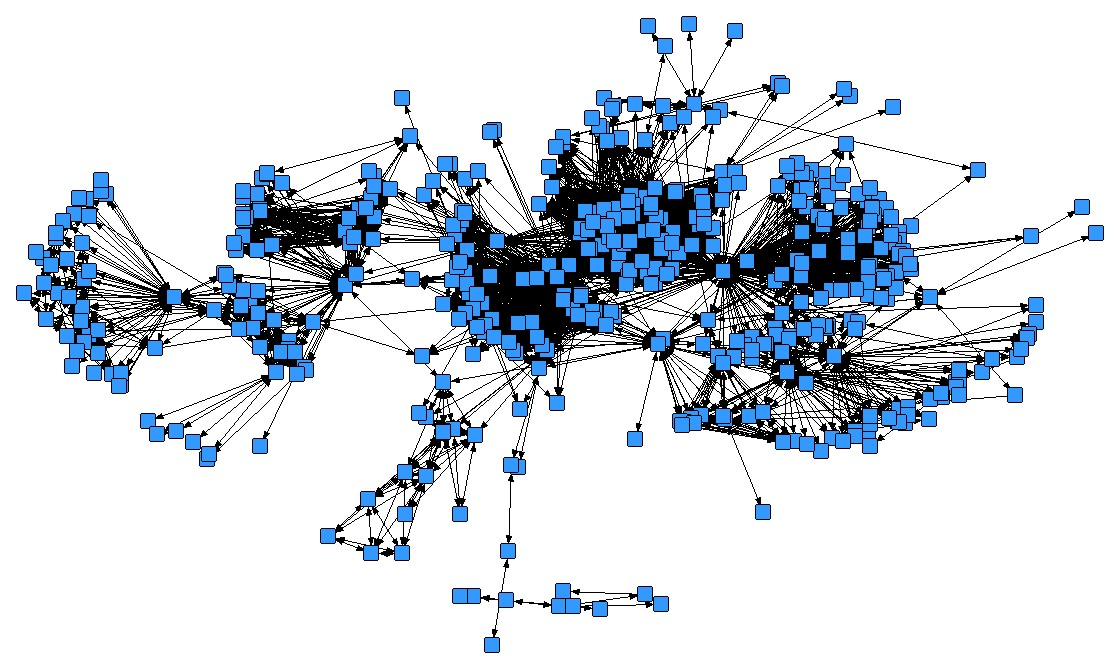
\includegraphics[width=\textwidth]{imgs/amigos-topicos.jpg}
\end{figure}

\begin{figure}[h!]
  \caption{A rede de atenção nas narrativas do A.M.I.G.O.S.}
  \centering
    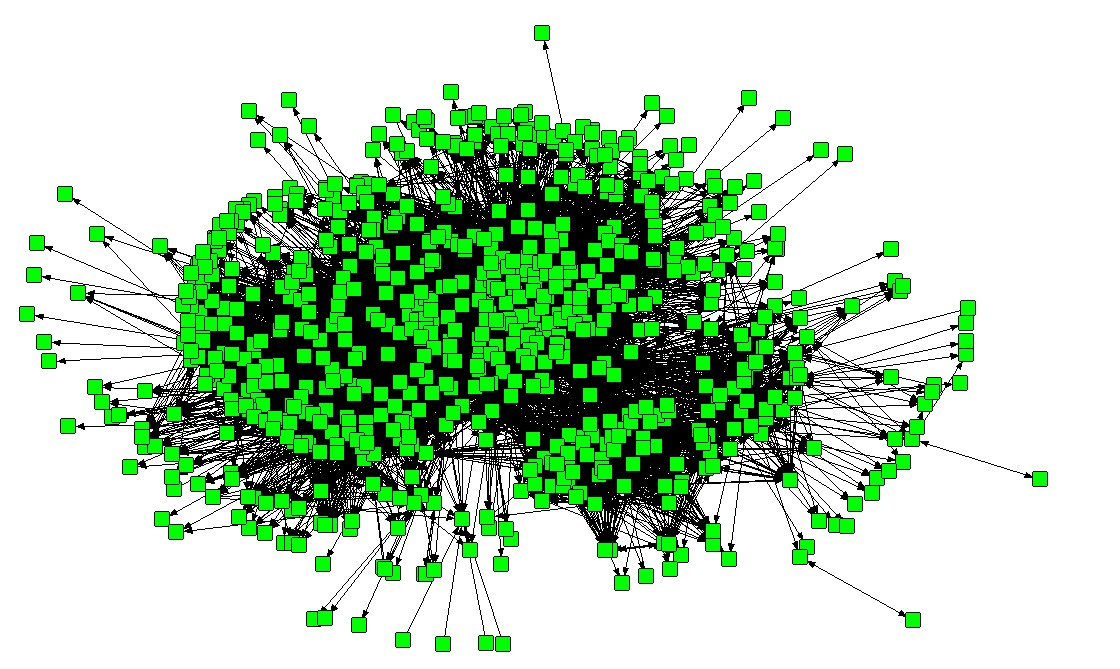
\includegraphics[width=\textwidth]{imgs/amigos-narrativas.jpg}
\end{figure}

\begin{figure}[h!]
  \caption{A rede de atenção total do A.M.I.G.O.S.}
  \centering
    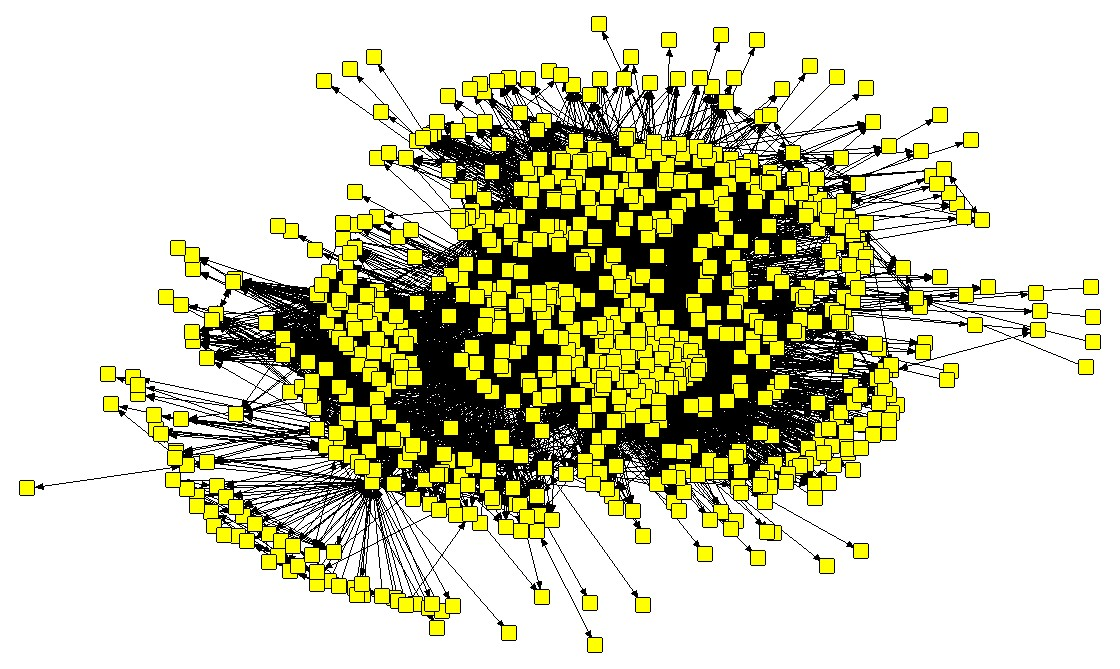
\includegraphics[width=\textwidth]{imgs/amigos-atencao.jpg}
\end{figure}

\begin{table}[htbp]
	\begin{boxedminipage}{\textwidth}
		Utilizamos a formalização descrita na seção \ref{sec:formalizacao} sobre a
		rede de teste do A.M.I.G.O.S. Os parâmetros foram:
		\begin{itemize}
		  \item $\alpha = 0.2$
		  \item $\beta = ^1/_\text{(quantidade da abrangência)}$
		  \item $\gamma = 0.5$
		\end{itemize}
		Foram consideradas os fórums e as narrativas (com seus comentários).
		Narrativas são similares aos \textit{posts} de \textit{blog} convencionais.
		Fizemos testes com várias possibilidades para $|i_k|$ pois a variância
		indicava muito ruído. Pode se ter como exemplo de ruído uma mensagem de
		fórum onde o autor copiou enorme lista com os nomes dos arquivos presentes na
		comunidade, nem o autor dedicou muito tempo ao copiar a lista, nem os outros
		membros devem ter dado muita atenção à lista inteira. Sendo assim, escolhemos
		um $|i_k|$ que desprezasse interações com quantidades de palavras muito
		destoantes. Fizemos $|i_k|=\tanh(0.5\lambda x)$ onde $x$ é a quantidade de
		fato de palavras e $\lambda=-\frac{\ln(10^{-4})}{\overline{x} + 5\sigma}$,
		$\overline{x}$ é a média e $\sigma$ é o desvio padrão, logo temos que pelo
		menos 95\% das interações encontram-se entre 0 e 0.9999.
		
		Foi coletado a rede usando apenas a interação por tópicos, depois por
		narrativas, depois as duas combinadas. A
		tabela~\ref{tab:comparacao_contato_atencao} apresenta uma comparação entre os
		quatro tipos de rede coletadas até agora.
		
% 		\large       % tamanho da fonte 
		\setlength{\arrayrulewidth}{2\arrayrulewidth}  % espessura da  linha
		\setlength{\belowcaptionskip}{10pt}  % espaço entre caption e tabela
		\caption{\it Comparação entre a rede de contatos e de atenção.}
		\centering   % tabela centralizada
		\begin{tabular}{| l | l | l | l | l |}
		\hline
		Métrica & Contatos & Fóruns & Narr. & Atenção \\ \hline
		Densidade & 0.0136 & 0.1861 & 0.05 & 0.05\\
		Reciprocidade & 0.5841 & 0.1120 & 0.83 & 0.79\\
		Coef. Cluster & 0.554 & 0.45 & 0.67 & 0.66\\
		Coef. Cluster Ponderada & 0.290 & 0.099 & 0.49 & 0.47\\
		Distância (geodésica) & 4.499 & 1.0340 & 2.54 & 2.63\\
		Coesão (Distância) & 0.183 & 0.983 & 0.43 & 0.41\\
		Largura (Distância) & 0.817 & 0.017 & 0.57 & 0.59\\
		Fitness (Núcleo/Periferia) & 0.257 & 0.0 & 0.44 & 0.44\\
		\hline
		\end{tabular}
		\label{tab:comparacao_contato_atencao}
		\flushleft
		\normalsize
		Nota-se uma maior adensamento da rede com encurtamento de caminhos nas redes
		de atenção. Porém enquanto a que foi formada a partir das interações nos
		fóruns tem menor coeficiente de \textit{clusterização} da rede com nenhum
		indicativo de padrão núcleo/periferia, a proveniente das narrativas tendência
		oposta. Pode-se dizer, que na rede do A.M.I.G.O.S. os fóruns descentralizam a
		distribuição da atenção, enquanto que as narrativas atuam em sentido
		contrário.
	\end{boxedminipage}
\end{table}

\section{critérios de escolha da representação}

Qual a rede ideal para o cálculo de proeminência? Não há resposta objetiva para
essa pergunta. Cada rede é uma representação de um fenômeno social que vai além
das ferramentas, mesmo sendo capaz de coletar e integrar todas as interações
digitais, as pessoas ainda vão ser capazes de tomar um café juntas e nossa visão
será apenas parcial. Sendo assim, é evidente que cada representação mensurada é
uma parte da informação e, portanto, capaz de descrever aspectos diferentes ou
não do fenômeno. São essas variações entre as representações de redes que
chamaremos de \textbf{critérios de escolha}.

Para enteder sua utilidade, um exemplo: imaginemos que ao final da análise
tenhamos duas ou mais representações da rede: uma textual e algumas não
textuais. Para cada uma encontramos valores diferentes de proeminência,
então qual usar? Colocando de outra forma, quanto de informação estarei perdendo
caso considere apenas uma delas? 

Esse é um problema bastante similar ao que estudiosos de aprendizagem de máquina
chamam de seleção de características (\textit{feature selection}) e que consiste
em decidir quais subconjunto de todas as variáveis possíveis que podem ser
utilizadas no treinamento da máquina são maximamente dependentes do resultado
esperado, ou seja, é maximamente relevante e minimamente redundante. No nosso
caso, porém, como afirmado acima, não há a rede \textbf{certa} e por isso a
relevância de todas elas são iguais. O que podemos procurar, portanto, é um
subconjunto com minimize a redundância. De acordo com o mais recente algoritmo
de mRMR (\textit{minimal-redundancy-maximal-relevance}) define-se a mínima
redundância como:

\begin{equation}
\label{def:min_redun}
\min R(S), R = \frac{1}{|S|^2}\sum_{x_i, x_j \in S}I(x_i, x_j)
\end{equation}

Onde $S$ é um subconjunto de características e $I(.)$ é a função de mútua
informação. Por definição, a função de mútua informação mede a correlação entre
duas variáveis aleatórias, porém, para o caso de redes sociais, o procedimento
comum é modelar cada par de ator como uma variável separada cujos valores
possíveis depende do tipo da rede. Se considerássemos cada rede como uma única
variável que representasse a chance de dois atores quaisquer estarem ligados,
então estaríamos nos limitando a uma correlação de suas densidades, o que de
forma nenhuma é interessante para nosso objetivo já que o cálculo de
proeminência varia consideravelmente a depender dos padrões das conexões,
mesmo em redes com densidade iguais.

Por esta razão, precisamos adaptar nossa função de mútua informação para
considerar as peculiaridades das redes sociais. Basicamente temos duas opções:
considerar a redundância das conexões ou calcular a proeminência para cada
rede e a partir daí determinar sua correlação. 

\subsection{Redundância das conexões}

Uma conexão é redundante quando pode ser encontrada em mais de uma rede. Mais do
que isso, duas redes são redundantes quando além de compartilhar conexões também
compartilham determinados padrões como triângulos e subgrupos. As duas
famílias de ferramentas para acessar essa similaridade estrutural mais
desenvolvidas na literatura são: gráficos aleatórios exponenciais e procedimento
de atribuição quadrática, respectivamente $p*$ (\textit{exponential random
graphs}) e \textit{QAP} (\textit{quadratic assignment procedure}).

\subsubsection{redes discretas e/ou esparsas}

O primeiro é mais apropriado para redes binárias ou com valores discretos.
Consiste em criar um modelo exponencial para a criação de grafos aleatórios a
partir de um conjunto de parâmetros relacionados a \textbf{configurações} de
interesse. Uma configuração pode ser desde a presença de uma conexão, até a
quantidade de k-triângulos e outros padrões mais complexos. Cada configuração
tem um parâmetro relacionado que pode ser negativo, indicando que a rede é tem
tendência inversa à presença daquela configuração, nula representando a
indiferença e positiva para uma tendência de mesmo modo. Assim sendo, cada
parâmetro pode ser visto como tendências da rede em relação a, por exemplo:
densidade, reciprocidade e transitividade da rede quando suas configurações
relativas são respectivamente a presença de conexões, a mutualidade das
relações e a presença de triângulos. 

Modelos exponenciais de gráficos aleatórios tem a seguinte forma geral:

\begin{equation}
\label{def:p_star_geral}
\Pr(\textbf{Y} = \textbf{y})
=\left(\frac{1}{k}\right)\exp\left\{\sum_A\eta_Ag_A(\textbf{y})\right\}
\end{equation}

Onde (i) o somatório é sobre todas as configurações procuradas em \textbf{y};
(ii) $\eta_A$ é o parâmetro relacionado à configuração $A$; (iii)
$g_A(\textbf{y})=1$ se a configuração é observada em \textbf{y}, ou 0 de outra
forma; (iv) $k$ é uma constante de normalização que garante que
(\ref{def:p_star_geral}) é uma distribuição de probabilidades. O vetor de
parâmetros $\eta$ é estimado para o grafo a ser modelado, procurando maximizar
a sua probabilidade, iterativamente a partir de simulações com o método Monte
Carlo (\textit{Markov chain Monte Carlo maximum likelihood estimation}).

Voltando ao problema de minimizar a redundância, podemos considerar o vetor
$\eta$ no cálculo de ``informação mútua'' entre as redes, no sentido de que
redes possuem a mesma informação se compartilham conexões e tendências similares
ao aparecimento de padrões estruturais. Derivamos $I_D$ para redes discretas:

\begin{equation}
\label{def:MI_discreto}
I_D(x, y) =\frac{\sum_{i,j = 1}^n x_{ij}y_{ij}}{\sum_{i,j = 1}^n
y_{ij}\sum_{i,j=1}^n x_{ij}} \rho(\eta_x, \eta_y)
\end{equation}

Onde (i) o numerador é a quantidade de conexões presentes em ambas $x$ e $y$;
(ii) o denominador da fração é a soma de todas as conexões de $x$ e todas de
$y$; e (iii) é a correlação linear entre os parâmetros $\eta$ estimados para $x$
e os estimados para $y$. Substituindo (\ref{def:MI_discreto}) em
(\ref{def:min_redun}) temos um modelo para o conjunto de redes com mínima
redundância.

\subsubsection{redes contínuas densas}

Para rede contínuas, um segundo método pode ser utilizado para calcular a
correlação diretamente. O procedimento de atribuição quadrática (\textit{QAP})
recomenda um modelo linear para a correlação das redes, assim, temos que:

\begin{equation}
\label{def:linear_model_qap}
Y = \alpha X + \epsilon
\end{equation}

A probabilidade de que a correlação encontrada não seja apenas coincidência é
acessada através da permuta das colunas da matriz seguindo algoritmo apropriado.
Não é nosso objetivo nos aprofundar na especifidades do teste, apenas é pertinente
considerarmos a  utilização da correlação linear como valor para a informação
mútua em \ref{def:min_redun} para redes de valores contínuos densos.

\subsection{Correlação de Proeminência}

O critério anterior busca relacionar as características da rede em busca de
informações redundante, porém também é interessante observar a relação que há
entre o produto final da análise das redes que são as medições de proeminência.
Para esse fim utilizaremos também a correlação linear de Pearson de forma que
duas redes podem estar positivamente relacionadas, aparentemente independentes
ou negativamente relacionadas. Um critério baseado na proeminência pode
correlacionar redes estruturalmente bastante diferentes, mas que resultam no
sobressaimento dos mesmos atores em termos de importância. Porém, se o objetivo
for minizar a redundância do ponto de vista da ordenação final dos atores por
grau de proeminência para a utilização em outros algoritmos como por exemplo,
escolha de subconjunto ótimo para marketing viral, então talvez este critério
seja o mais apropriado.

\begin{table}[htbp]
	\begin{boxedminipage}{\textwidth}
	No caso do A.M.I.G.O.S. só temos duas representações da rede, a primeira 
	proveniente da interação não textual ``contatos'', a segunda é a união de duas
	interações textuais: fóruns e narrativas. Sendo assim, só podemos avaliar o
	quão diferentes são as redes e por isso mesmo, o quanto de informação vamos
	perder escolhendo uma ou outra.
	
	Como a rede de contatos é binária a correlação linear fica prejudicada devido a
	limitação do modelo em relação a dados tão dicotômicos (0 ou 1), porém não
	temos uma implementação disponível de um algoritmo de estimativa no modelo $p*$
	para a nova configuração e executamos um teste de correlação QAP entre as duas
	redes. Verificamos que a rede de contatos e de atenção possuem um coeficiente
	de correlação positiva de 0.27, que quer dizer que a chance de encontrarmos um
	laço entre dois atores em ambas as redes é de 27\%. A chance de uma correlação
	nessa proporção acontecer entre as redes considerando uma combinação aleatória
	é menor que 0.001 e $R^2$ de apenas 0.07, parte devido à dicotomia dos dados.
	
	Também realizamos um teste de regressão para as duas métricas de proeminência
	escolhidas, o índice de poder de Bonacich e o de \textit{betweeness} de
	Freeman. Encontramos nenhuma correlação entre as redes para o primeiro,
	indicando que quanto a influência ambas as redes são bastante distintas. Já em
	termos de centralidade, pudemos verificar uma correlação positiva de 0.47, com
	$R^2=0.22$ e $p. < 0.0001$.
	
	Com essas medidas podemos avaliar melhor a perda de informação que teremos ao
	escolher apenas uma das redes. Não há necessidade de buscar um subconjunto de
	redes que minimize a redundância por que só temos 2 redes.
	
	\end{boxedminipage}
\end{table}

\subsection{Conclusão e trabalhos futuros}

Cada dia mais e mais interações entre pessoas ocorre em meio digital, essas
interações podem proporcionar a mensuração de diversas representações da rede
social que interliga estes indivíduos. O resultado deste processo pode alimentar
novas ações no campo do marketing, modelos sobre disseminação de idéias,
doenças e reconhecimento de especialistas. A seleção apropriada de medianeiros
para o recolhimento 

\title{PARTE II}

\section{outros problemas em relação às métricas de proeminência}

Voltando a questão da proeminência, mesmo que consigamos definir os medianeiros,
identificar os tipos de interação, mensurar a atenção investida e formalizar uma
rede direcionada e valorada, ainda assim teremos que a métrica pode não ser
significativa dependendo da parte da rede sobre o qual foi aplicada. Nota-se que
o que as métricas de proeminência fazem é verificar o envolvimento do nó com os
possíveis caminhos da rede como grafo. Nesse sentido, podemos dividir as
métricas em dois grandes grupos: as radiais que medem seu envolvimento nas
extremidades do caminho e as mediais que a fazem nos elos intermediários.

[relações intertextuais entre os atores para a formação de comunidades de
prática.]

Quando tudo o que temos é a rede para medirmos proeminência em atores de redes
sociais digitais precisamos de uma maneira de medir sua aplicabilidade.


% \center
\begin{tabular}{| l | l |}
\hline
Métrica & Valor \\ \hline
Densidade & 0.0136 \\
Reciprocidade & 0.5841 \\
Coef. Cluster & 0.554 \\
Coef. Cluster Ponderada & 0.290 \\
Distância (geodésica) & 4.499 \\
Coesão (Distância) & 0.183 \\
Largura (Distância) & 0.817 \\
Fitness (Núcleo/Periferia) & 0.257 \\
\hline
\end{tabular}

% \flushleft
A densidade, distância, coesão e largura nos diz que a rede é esparsa. O
coeficiente de clusterização mostra que apesar de que atores com poucos contatos
tem uma vizinhança relativamente interconectada, quanto maior a sua vizinhança,
menor a interconexão. Finalmente, o algoritmo de detecção de Núcleo/Periferia
encontrou baixa adequação. Todas essas métricas indicam que temos diversos
subgrupos dentro da rede e que ela está longe de se assemelhar a uma comunidade
de prática. Numa situação assim, [métricas mediais perdem força descritiva da
influência do ator na rede como um todo TODO: revisar isso aqui].

Por outro lado, herdamos alguns problemas dessa escolha também. O primeiro é um
problema tradicional na área: como saber se as medidas usadas por cada
membro para dar notas às relações são iguais (ou minimamente relacionáveis)? De
um ponto de vista filosófico, vale a pena até perguntar se essa pergunta faz
sentido. Mas para contornar esse problema acabamos esbarrando em um outro, que é
como as interações observadas combinam para formar uma representação confiável
da rede, uma que produza resultados apreciáveis para a análise de influência? 

Essa e outras questões como a forma de medir o impacto dependem do tipo de
interação considerada.  Para tal, destacamos a necessidade de uma
\textbf{tipologia das interações} digitais, sobre a qual estruturaremos considerações sobre sua combinação.

Entender e recontar os significados nas interações humanas tem sido o objetivo
das ciências sociais como a etnografia e antropologia. Para trazer respostas ao
nosso problema, nós precisamos buscar na etnografia digital uma base para 

\begin{wrapfigure}{r}{2in}
\begin{boxedminipage}{2in}
No estudo de caso realizado, foi considerada o site de relacionamento Amigos do
C.E.S.A.R. Composto em sua maioria por colaboradores do mesmo, a rede se
configura, portanto, como uma comunidade de prática, i.e. voltada para o
compartilhamento e a colaboração em torno de um foco comum, no caso
desenvolvimento de software. O ambiente foi aberto à pesquisa e por isso podemos
considerar que foi realizada uma análise intrínseca. Todas as informações
utilizadas são também informações públicas na rede.
\end{boxedminipage}
\end{wrapfigure}

\cite{Spertus2005} - similaridade em orkut

\section{Sobre Proeminência}

Proeminência é a característica dos relacionamentos de um ator que o põe em
evidência para outros atores na rede \cite{Wasserman}. A proeminência,
academicamente, foi separada em dois aspectos: centralidade e prestígio.
Centralidade é como o ator se posiciona na rede, sua interação e envolvimento com
os outros. Prestígio é como os outros atores se posicionam em relação a ele, como
interagem e envolvem-se com ele \cite{Knoke1983}.

Nosso objetivo, identificar atores chaves para processos de influência da rede,
está relacionado diretamente com o conceito de proeminência de forma que podemos
dizer que a usaremos como uma aproximação da influência do ator na transmissão de
conhecimento, inovações e opiniões pela rede. Por estes motivos, cuidado especial
deve ser tomado sobre a forma como calcularemos a proeminência e que
características são esperadas da representação da rede que será mensurada.

Durante décadas pesquisadores de redes sociais se debruçaram sobre o estudo da
proeminência, desenvolvendo inúmeras métricas que conjuntamente são chamadas de
métricas de centralidade. Quando calculadas considerando os caminhos que
\textbf{saem} do ator, referem-se a sua centralidade propriamente dita. Quando
considera-se os caminhos que \textbf{chegam} no ator, referem-se ao seu
prestígio. Não obstante tenha o comum senso de que essas métricas referem-se de
alguma forma à proeminência do ator, a forma específica tem ficado a cargo de
cada pesquisador que já atribuiu ao seu resultado interpretações como autonomia,
controle, risco, influência, corretagem (\textit{brokerage}), independência,
etc.

Freeman revisou as métricas existentes à época \cite{Freeman1979} e as compilou
em três principais centralidades: por grau, por proximidade (\textit{closeness})
e por intermediação (\textit{betweenness}). Interpretando seus resultados em
relação ao quanto o grafo se aproxima de uma estrutura de estrela
(Figura~\ref{fig:star}), sua visão de centralização ideal, onde suas métricas
alcançam o máximo.

\begin{figure}[h!]
  \caption{Gráfico estrela}
  \label{fig:star}
  \centering
    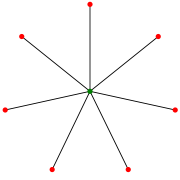
\includegraphics[width=0.3\textwidth]{imgs/star.png}
\end{figure}

Recentemente, Borgatti e Everett \cite{Borgatti2006} nos ofereceram uma
outra reposta para a questão: O que as métricas de centralidade medem? E
chegaram a conclusão que todas elas investigam o relacionamento do nó com os
possíveis caminhos do grafo. Em sua tipologia para a classificação das
métricas de centralidade, propõem quatro dimensões: tipo do caminho,
propriedade do caminho, tipo do envolvimento e forma de agregação. Em outras
palavras, toda métrica de centralidade é uma forma de agregar uma propriedade
dos caminhos de determinado tipo em que o nó tem um determinado envolvimento.
Das quatro dimensões, duas são de maior importância: propriedade do caminho e
tipo de envolvimento. 

\subsection{Tipo de envolvimento} 

O tipo de envolvimento é a dimensão de classificação proposta por Borgatti que
se traduz na maior variância nos resultados. Pode ser de dois tipos: radial ou
medial.

Métricas radiais são as que analisam os caminhos em que o nó está numa das
pontas, ou seja, que saem ou chegam nele. Exemplos de métricas radiais são as
centralidades de grau e proximidade de Freeman. A análise de Borgatti et al veio
confirmar o que as evidências empíricas já sugeriam, que as métricas radiais
representam a parcela de responsabilidade que o nó tem na coesão total da rede e
que, por este motivo, se enfraquecem a medida que a rede não se adequa ao padrão
de núcleo-periferia \cite{Nakao1990}.

Já as ditas mediais analisam os caminhos que passam pelo nó, classificando-o em
seu papel de \textit{gateway} entre partes da rede. O \textit{betweenness} de
Freeman é um exemplo de métrica medial. São mais estáveis em relação à
característica de núcleo-periferia, por outro lado tendem a dar maior importância
a atores que conectam grupos distintos, mas que se encontram na periferia dos
mesmos.

Os dois tipos são complementares e mais de uma métrica devem ser combinadas
(\cite{Stephenson1989}; \textit{Apud} \cite{Wasserman}). Pelo fato de que
usaremos métricas radiais de centralidade para estimar a influência do ator na
rede, já é possível derivarmos uma primeira restrição sobre a representação que
será mensurada:
\paragraph{
\emph{Quanto mais próximo a representação estiver do modelo de núcleo-periferia,
melhor será a aplicabilidade das métricas radiais de centralidade.}}

\subsection{Propriedade do caminho}

Borgatti define dois tipos de propriedade: distância e volume. A
propriedade do tipo distância mais comum é a geodésica que é a quantidade de
arcos presentes no menor caminho entre um ator e outro. Volume refere-se à
quantidade de caminhos entre os nós. As centralidades por grau e
\textit{betweenness} são exemplos de métricas que usam o volume dos caminhos,
enquanto que \textit{closeness} usa distância.

O critério de escolha depende da aplicação. Para o nosso caso, queremos modelar
o efeito da influência entre os pares na transmissão de informação. Nesse
sentido, quanto mais atores próximos estiverem tentando convencer alguém de
algo, maior será sua influência sobre este \cite{Watts2007}. Daí temos,
naturalmente, a preferência sobre métricas relacionadas a volume, no lugar de distância, já que
representa diretamente a quantidade de caminhos que existem entre os nós.

\subsection{Métricas de proeminência}

Escolhemos duas medidas para a análise de influência neste trabalho, uma para
centralidade e outra para prestígio. Ambas são do tipo volume, isto é, medem a
quantidade de caminhos, o que representa melhor o fenômeno de pressão social na
difusão de inovações. Para centralidade, utilizaremos a métrica medial
\textit{flow betweenness} que expande o conceito de \textit{betweenness} para
grafos não-binários \cite{Freeman1991} levando em consideração não apenas
geodésicas mas todos os caminhos que passam pelo ator, utilizando o peso das
arestas para medir a ``vazão'' que ``flui'' pelo mesmo. Para prestígio,
escolhemos a métrica radial de poder de Bonacich \cite{Bonacich1987} que
considera a soma dos caminhos que chegam ponderada pelo poder dos atores que a
compõem.

A interpretabilidade de tais métricas está diretamente relacionada com o que está
sendo medido na representação da rede. É fácil perceber o que o poder de Bonacich
significa se o arco do ator $i$ para o ator $j$ quer dizer que $i$ buscou os
conselhos de $j$. Por esta razão derivamos uma segunda restrição:

\paragraph{\emph{Quanto melhor a representação capturar a força dos
relacionamentos, tanto melhor será a aplicabilidade das métricas de proeminência;
Falhar em estimar a força das conexões levará a seleção de atores chaves em uma
miríade de interações irrelevantes. Da mesma forma, representar as conexões de
forma binária pode causar o enviesamento da rede ou para a superestimação de sua
força ou para a subestimação da mesma.}}

\cite{Cooper1997} e \cite{Silverstein2000} - artigo doido sobre formas de
encontrar relacao causal entre variaveis, pode ser usado para dizer que tal
influencia causou tal reacao

\cite{Friedman1999} - traz um modelo interessante baseado em probabilidade da
relacao para aprender relacoes entre atributos de atores, baseado em sua
aparicao estatistica no banco de dados, pode ser util usar isso para ajudar na
mensuracao

\begin{table}[htbp]
	\begin{boxedminipage}{\textwidth}
Para o estudo de caso da rede A.M.I.G.O.S. vamos começar analisando a rede
decorrente das conexões explícitas da rede: os contatos. Contatos são atores
explicitamente adicionados através da ferramenta, constituindo uma interação
não-textual individual-básica. Foram coletadas as interações de 1247 atores
representadas em um digrafo. Desses, 720 formam o componente principal do
digrafo (o maior subgrafo fracamente conexo) e removendo os que se conectam a
apenas 1 indivíduo temos 618 atores e 5180 conexões.
		\large       % tamanho da fonte 
		\setlength{\arrayrulewidth}{2\arrayrulewidth}  % espessura da  linha
		\setlength{\belowcaptionskip}{10pt}  % espaço entre caption e tabela
		\caption{\it Os 10 mais bem posicionados em Proeminência no A.M.I.G.O.S.}
		\centering   % tabela centralizada
		\begin{tabular}{| l | c |}
			\hline
			Ator & Centralidade \\ \hline
			8 & 0.230 \\
			135 & 0.136 \\
			1037 & 0.136 \\
			541 & 0.132 \\
			3 & 0.119 \\
			675 & 0.111 \\
			201 & 0.106 \\
			542 & 0.069 \\
			614 & 0.054 \\
			838 & 0.051\\
			\hline
		\end{tabular}
		\begin{tabular}{| l | c |}
			\hline
			Ator & Prestígio \\ \hline
			553 & 138.361 \\
			571 & 137.627 \\
			569 & 133.475 \\
			581 & 131.738 \\
			586 & 126.468 \\
			555 & 125.683 \\
			609 & 121.362 \\
			598 & 118.524 \\
			575 & 112.545 \\
			611 & 102.776 \\
			\hline
		\end{tabular}
		\label{tab:acontccent}
\flushleft
\normalsize
Na tabela~\ref{tab:acontccent} apresentamos o cálculo da centralidade
(\textit{Betweeness}) de Freeman e do prestígio (\textit{Power}) de Bonacich.
É notável que não há uma correlação entre as duas medidas e que os atores mais
centrais não são os atores com maior prestígio. Temos pouca informação externa
da rede sobre os atores mas é possível notar que no primeiro grupo (mais
central) estão presentes alguns pesquisadores-chefe da comunidade e que por isso
conectam grupos relativamente separados na rede. Já uma análise de clusterização
mostra que no segundo grupo (maior prestígio) estão membros de clusters
densamente conectados, o que explica terem sido escolhidos por muitos outros
atores que por sua vez foram escolhidos por muitos outros e assim
sucessivamente.

	\end{boxedminipage}
\end{table}
\clearpage
\begin{figure}[h!]
  \caption{A rede de contatos no A.M.I.G.O.S.}
  \centering
    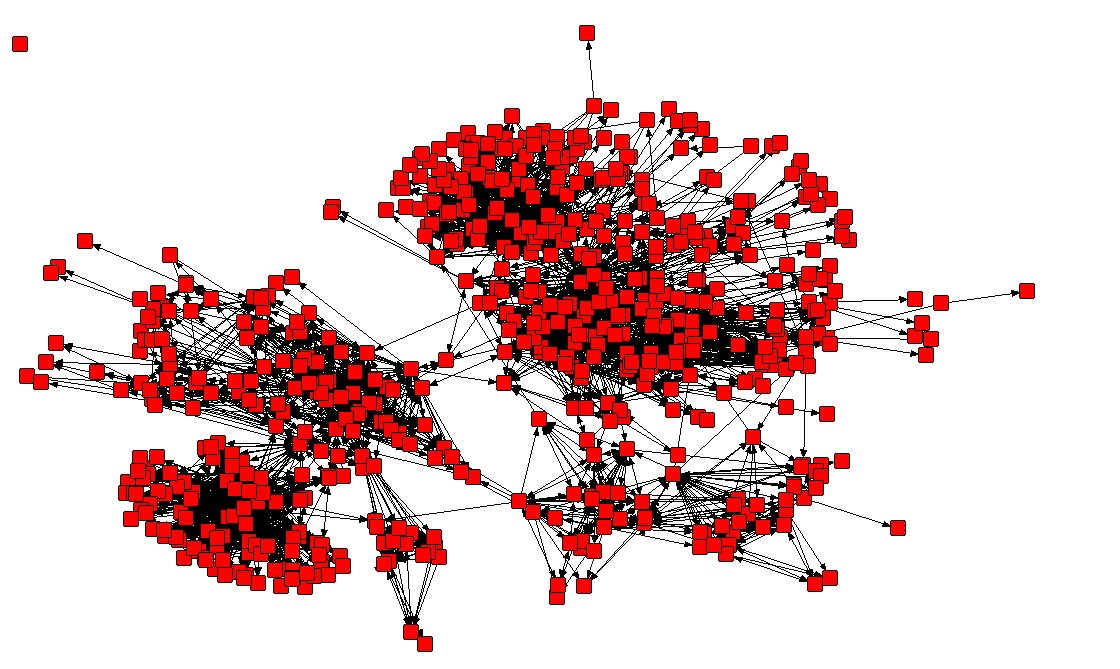
\includegraphics[width=\textwidth]{imgs/amigos-contatos.jpg}
\end{figure}


\bibliographystyle{alpha}
\bibliography{references}
\end{document}
